\white{North Dakota Signature Event Overview: (November 2, 2024)}
\chapterauthor{Caleb Bachmeier}
\info{November 2, 2024}{North Dakota Signature Event Overview}{Caleb Bachmeier}
\textbf{Goal:} Analyze the tournament in Grand Forks, North Dakota
\section*{General Tournament Information}
\begin{itemize}
    \item \textbf{Tournament Name:} The North Dakota VEX V5 Robotics Competition Signature Event, Presented by Bifrost
    \item \textbf{Date:} 1st and 2nd of November, 2024
    \item \textbf{Location:} Grand Forks, North Dakota 
    \item \textbf{Winning Teams:} 7686A - 7686X
\end{itemize}

\section*{Performance Information}
\begin{itemize}
    \item \textbf{Record for Qualification Matches}: 3/7/0
    \item \textbf{Alliance Selection:} 7686A
    \item \textbf{Awards:} Tournament Champions 
\end{itemize}

\subsection*{Qualification: 3}
\subsubsection*{Prediction}
For this (and future) tournaments we will be using a website called VRC Data Analysis. This website requires it's own chapter on it, but the basics are that it takes Microsoft's True Skill Rankings, and uses an API to determine the outcome of a match. We will show the predictions for each match. One bad thing about this, is that it doesn't take into account how well the Alliance works together, i.e what the robot does. Although, it still works great.
\begin{figure}[H]
    \centering
    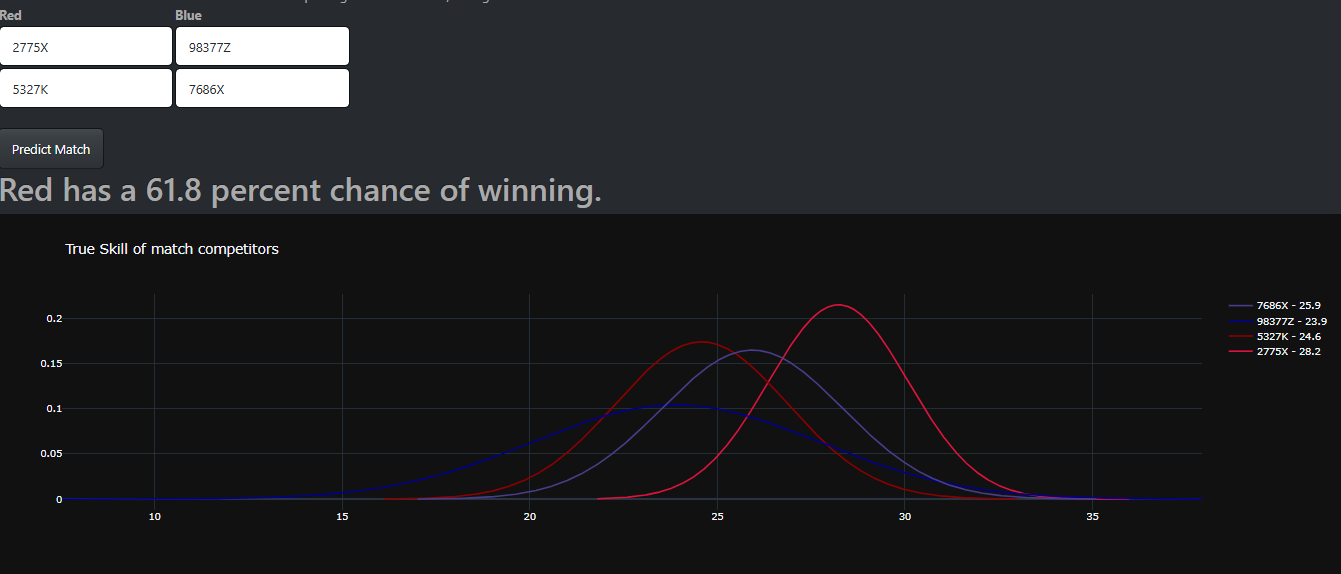
\includegraphics[width=0.8\linewidth]{images/Q3ND.png}
    \caption{Qualification 3 Predictions}
    \label{fig:Qual-3-ND}
\end{figure}
\begin{itemize}
    \item \textbf{Blue Alliance:} 98377Z - 7686X
    \item \textbf{Red Alliance:} 2775X - 5327K
    \item \textbf{Score}: \colorbox{cyan}{14}
    \colorbox{red}{38}
    \item \textbf{Autonomous Winner:} Red
    \item \textbf{How the match went}: In the Autonomous Period we successfully scored two blue Rings on a Stake, our Alliance partner didn't have an Autonomous Program. Unfortunately for us, 5327K had a program that could score three Rings, so we lost that. In Driver Control, Red quickly scores a Ring on their Alliance Wall Stake. Both us and our opponents filled a Mobile Goal with our respective colors and put it in their corners and protected, we protected while 98377Z tried to bully 2775X away from scoring more rings. Eventually, 5327K left their corner to score more points, leaving their corner exposed. This is a great opportunity for our partner to take the Red Mobile Goal out of the Positive Corner, but they didn't have a MoGo mechanism to do that. In the last fifteen seconds Red filled up two entire Mobile Goals, we couldn't prevent them.
    \item \textbf{What We Can Learn:} We should have been bullying 2775X, and our partner should have been protecting our goal. If we would have done this we likely would have been able to take the Red Mobile Goal out of the Positive Corner
\end{itemize}

\subsection*{Qualification: 21}
\subsubsection*{Prediction}
\begin{figure}[H]
    \centering
    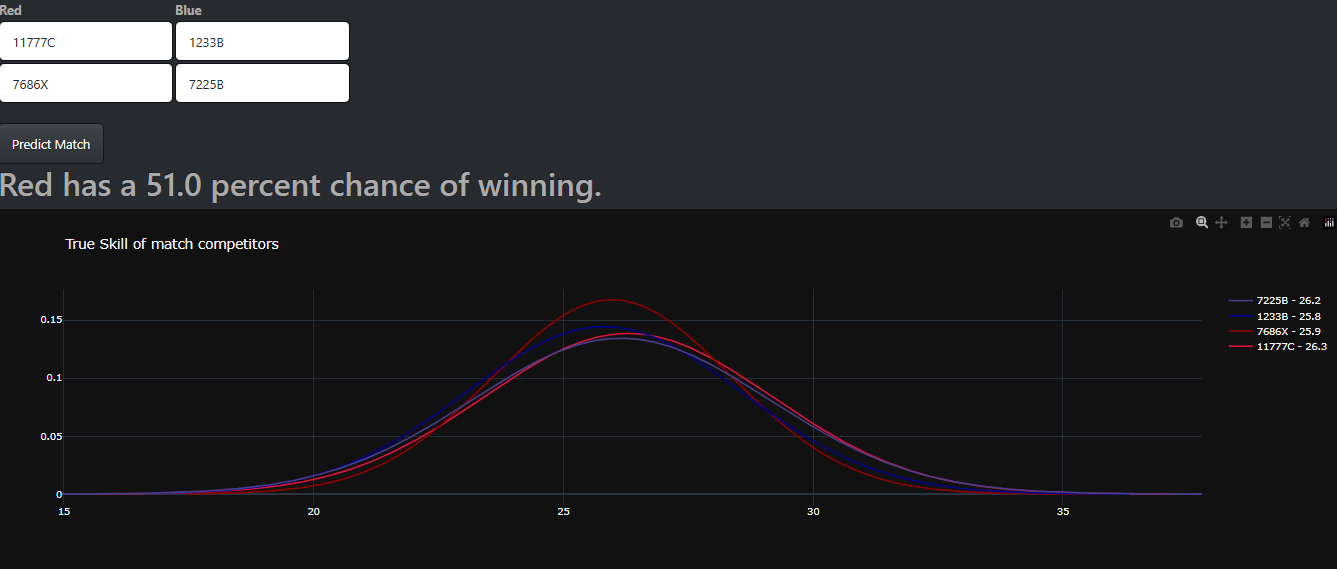
\includegraphics[width=0.8\linewidth]{images/Q21ND.png}
    \caption{Qualification 21 Prediction}
    \label{fig:Qual-21-ND}
\end{figure}
\begin{itemize}
    \item \textbf{Blue Alliance:} 1233B - 7225B 
    \item \textbf{Red Alliance:} 11777C - 7686X
    \item \textbf{Score}: \colorbox{cyan}{27}
    \colorbox{red}{22}
    \item \textbf{Autonomous Winner:} Red 
    \item \textbf{How the match went}: In the Autonomous Period our Autonomous worked again and we scored two Red rings. In Driver Control both teams got a full Mobile Goal and but them in their respective Positive Corners. Once the Endgame Period started we put a blue Mobile Goal in the Negative Corner and fought to keep it in, but 1233B came over and knocked over the Mobile Goa at the last second.
    \item \textbf{What We Can Learn:} We need to protect Mobile Goals in corners better because teams can just come and destroy our hard work
\end{itemize}

\subsection*{Qualification: 30}
\subsubsection*{Prediction}
\begin{figure}[H]
    \centering
    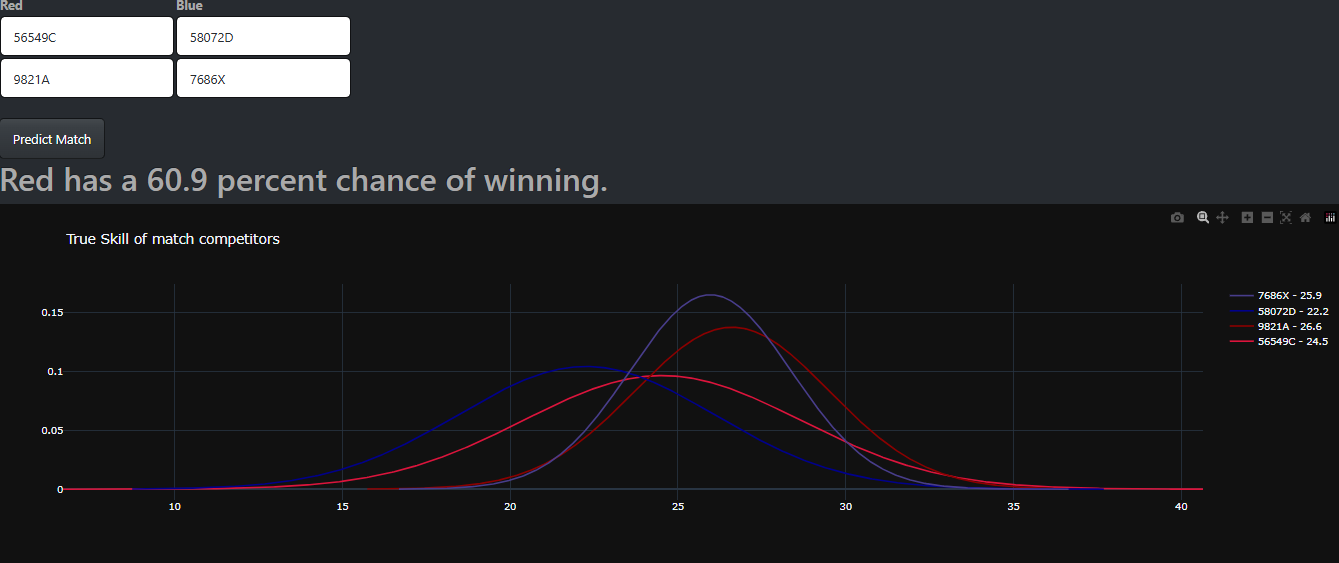
\includegraphics[width=0.8\linewidth]{images/Q30ND.png}
    \caption{Qualification 30 Prediction}
    \label{fig:Qual-30-ND}
\end{figure}
\begin{itemize}
    \item \textbf{Blue Alliance:} 58072D - 7686X
    \item \textbf{Red Alliance:} 56549C - 9821A
    \item \textbf{Score}: \colorbox{cyan}{15}
    \colorbox{red}{18}
    \item \textbf{Autonomous Winner:} Tie
    \item \textbf{Our Strategy:} 58072D are going to be on the defensive, they have proven to be good at it in the past. 56549C has a redirect mechanism and 9821A has a herobot, they can't score.
    \item \textbf{How the match went}: Autonomous: Nobody moved, the entire Autonomous period, which was very odd, so that resulted in a tie. Drivers: Our drivers period was very good, 58072D stoped 56549C from scoring. We eventfully got a Mobile Goal in the corner and won the match.
\end{itemize}

\subsection*{Qualification: 68}
\subsubsection*{Prediction}
\begin{figure}[H]
    \centering
    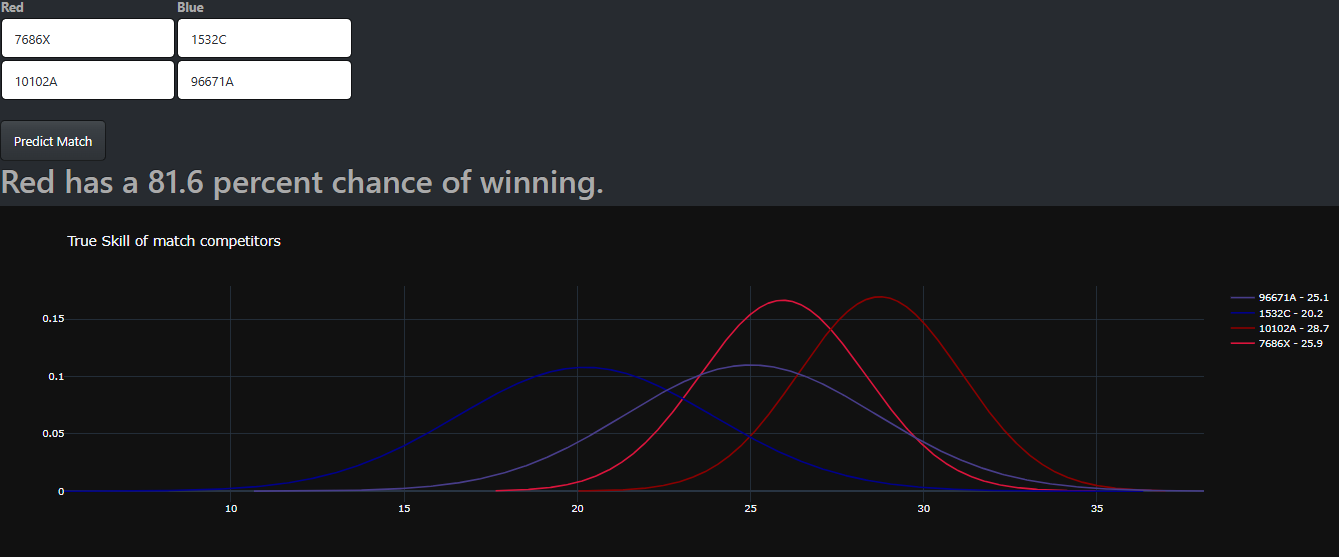
\includegraphics[width=0.8\linewidth]{images/Q68ND.png}
    \caption{Caption}
    \label{fig:enter-label}
\end{figure}
\begin{itemize}
    \item \textbf{Blue Alliance:} 1532C - 96671A
    \item \textbf{Red Alliance:} 7686X - 10102A
    \item \textbf{Score}: \colorbox{cyan}{32}
    \colorbox{red}{30}
    \item \textbf{Autonomous Winner:} Red
    \item \textbf{Our Strategy}: The strategy for this match is defend the positive corner with the Mobile Goal we will fill during the Autonomous Period while they try to score.
    \item \textbf{How the match went}: Autonomous Period: 10102A has a five ring scoring Negative side autonomous program, while our Autonomous succeed making us win the autonomous bonus. Driver: We quickly went over to the positive corner and placed our Mobile Goal there. 10102A filled up a Mobile Goal and put it in the other Positive Corner. Making the Red Alliance win the match
\end{itemize}

\subsection*{Qualification: 78}
\subsubsection*{Prediction}
\begin{figure}[H]
    \centering
    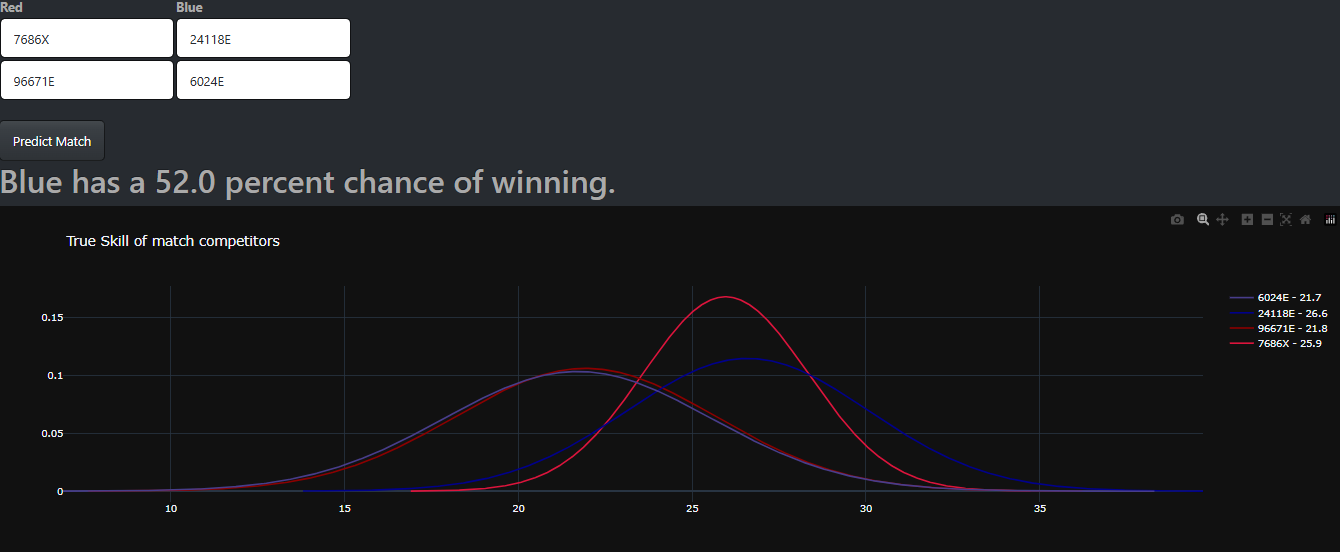
\includegraphics[width=0.8\linewidth]{images/Q78ND.png}
    \caption{Caption}
    \label{fig:enter-label}
\end{figure}
\begin{itemize}
    \item \textbf{Blue Alliance:} 24118E - 6024E
    \item \textbf{Red Alliance:} 96671E - 7686X
    \item \textbf{Score}: \colorbox{cyan}{35}
    \colorbox{red}{25}
    \item \textbf{Autonomous Winner:} Blue
    \item \textbf{Our Strategy}: 7686X will defend their Mobile Goal in the Positive Corner while 96671E fills up their Mobile Goal and places it in the other Positive Corner
    \item \textbf{How the match went}: Autonomous Period: 96671E had a three Ring Autonomous, but 7686X's didn't work for some reason, making Blue get the Alliance Bonus. Driver: Blue quickly gets top ring on both Neutral Stakes, while 7686X rushes the Positive Corner. 7686X remains in the corner until fifteen seconds remain, when they get top Ring on both Neutral Stakes.
\end{itemize}

\subsection*{Qualification: 84}
\subsubsection*{Prediction}
\begin{figure}[H]
    \centering
    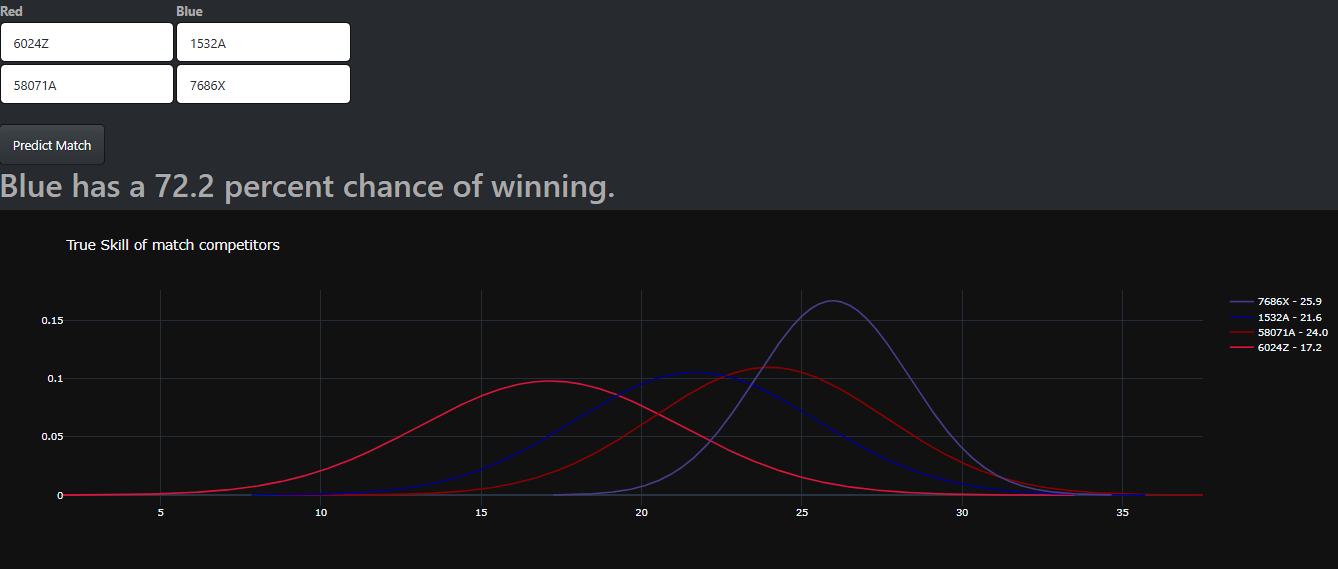
\includegraphics[width=0.8\linewidth]{images/Q84ND.png}
    \caption{Caption}
    \label{fig:enter-label}
\end{figure}
\begin{itemize}
    \item \textbf{Blue Alliance:} 7686X - 1532A 
    \item \textbf{Red Alliance:} 6024Z - 58071A
    \item \textbf{Score}: \colorbox{cyan}{22}
    \colorbox{red}{10}
    \item \textbf{Autonomous Winner:} Tie  
    \item \textbf{How the match went}: Autonomous Period: We only got one Ring scored, while Red got one too, so it was a Autonomous was a tie. Driver: We got two full Mobile Goals in the corner, so we won.
\end{itemize}

\subsection*{Qualification: 94}
\subsubsection*{Prediction}
\begin{figure}[H]
    \centering
    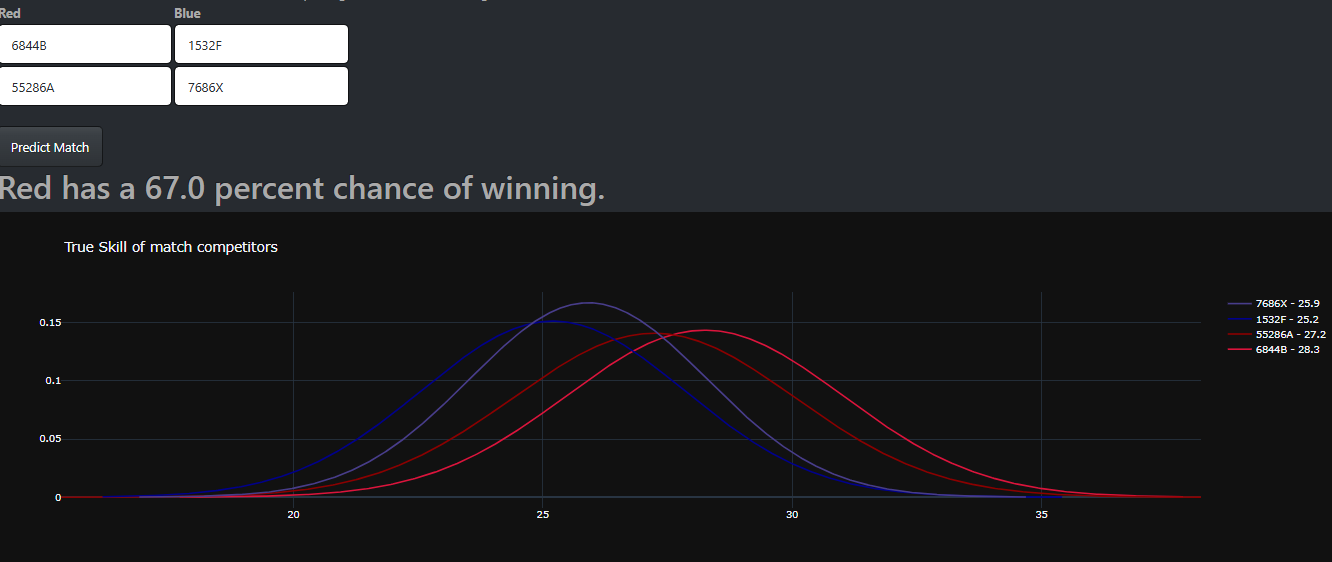
\includegraphics[width=0.8\linewidth]{images/Q94ND.png}
    \caption{Caption}
    \label{fig:enter-label}
\end{figure}
\begin{itemize}
    \item \textbf{Blue Alliance:} 7686X - 1532F
    \item \textbf{Red Alliance:} 6844B - 55286A
    \item \textbf{Score}: \colorbox{cyan}{12}
    \colorbox{red}{40}
    \item \textbf{Autonomous Winner:} Red
    \item \textbf{How the match went}: Autonomous Period: Blue only scored one Ring, Red scored five, so they were the obvious winner. Driver: Red got two full Mobile Goals and camped the Positive Corners with them. Blue ended up getting both top rings on the Neutral Stakes. 
\end{itemize}
\section*{Eliminations}
\subsection*{Alliance Selection}
Our main choices were 10102A, C, X, and 96671G. We decided on 96671G, they seemed like a well rounded team. Unfortunately for 7686A, their Alliance Partners got chosen and declined, so they couldn't chose each other, so 7686A chose us, which was definitely good for us.
\subsection*{Round of 16}
\subsubsection*{Prediction}
\begin{figure}[H]
    \centering
    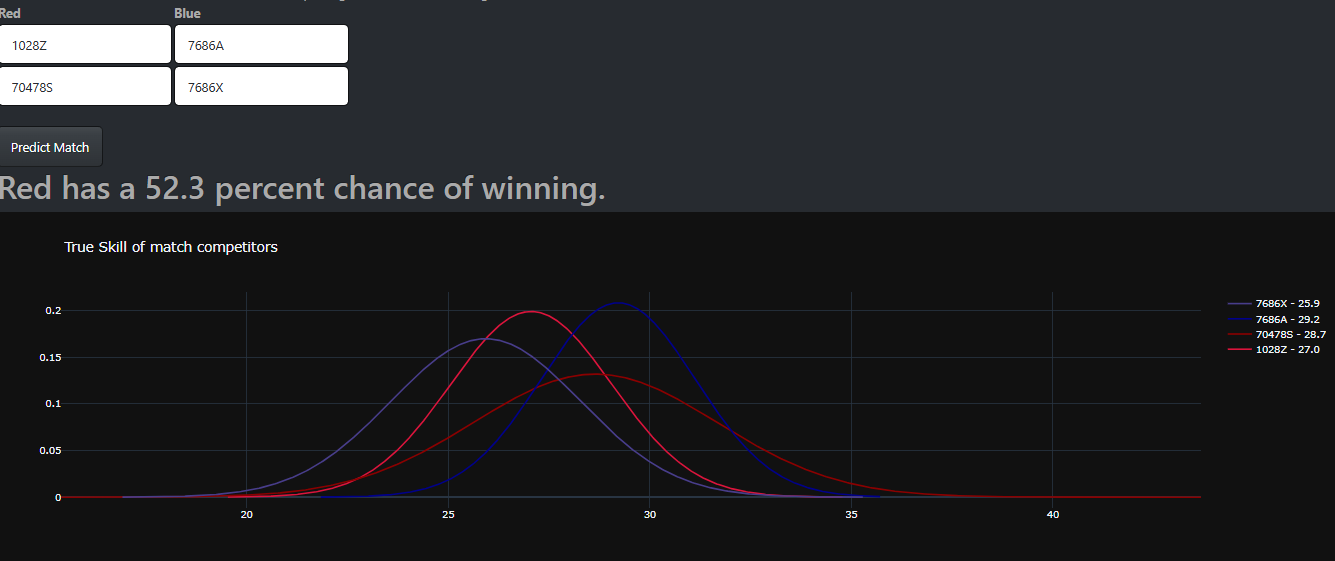
\includegraphics[width=0.8\linewidth]{images/R16ND.png}
    \caption{Caption}
    \label{fig:enter-label}
\end{figure}
\begin{itemize}
    \item \textbf{Blue Alliance:} 7686A - 7686X
    \item \textbf{Red Alliance:} 1028Z - 70478S
    \item \textbf{Score}: \colorbox{cyan}{32}
    \colorbox{red}{22}
    \item \textbf{Autonomous Winner:} Tie
    \item \textbf{Our Strategy:} Our strategy will be the same for all of our elimination matches. After Autonomous, 7686A will give us their Mobile Goal while we stay in our corner and try to fill up our Mobile Goal. 
    \item \textbf{How the match went}: Autonomous Period: We got one Blue Ring, and they got one Red Ring, so it was a tie. Driver: 7686A and X switched Mobile Goals, X filled theirs and put it in the Positive Corner, but A couldn't get an opening to put it in their Positive Corner. In the last fifteen seconds we scored one top Ring on a Neutral Stake, closest match of the day so far.
\end{itemize}

\subsection*{Quarterfinals}
\subsubsection*{Prediction}
\begin{figure}[H]
    \centering
    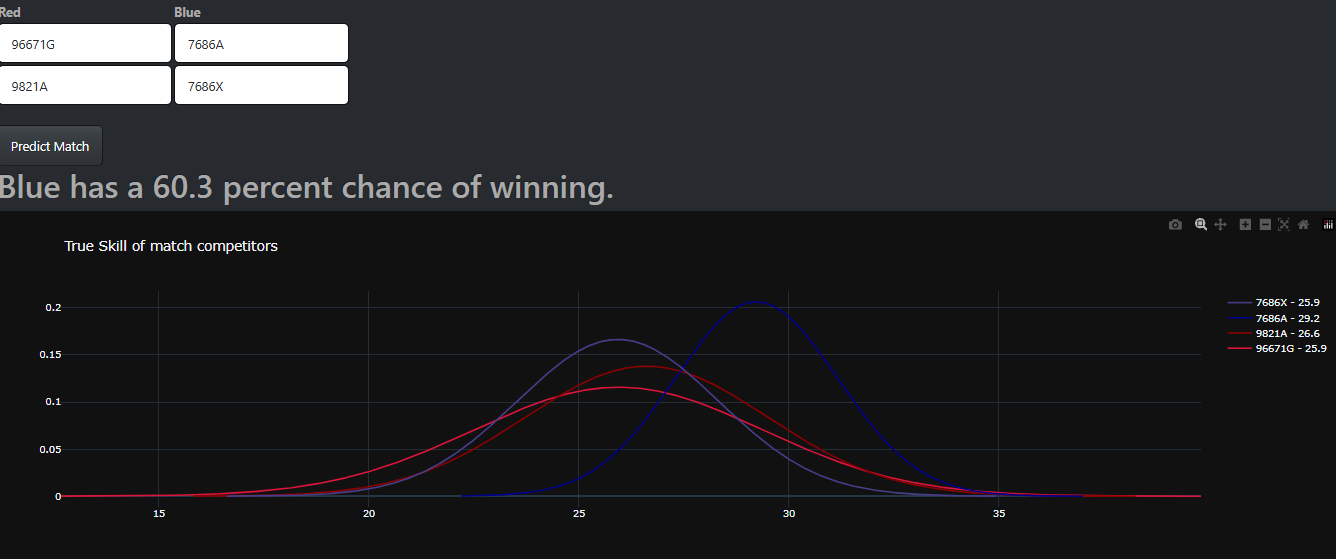
\includegraphics[width=0.8\linewidth]{images/QFND.png}
    \caption{Caption}
    \label{fig:enter-label}
\end{figure}
\begin{itemize}
    \item \textbf{Blue Alliance:} 7686A - 7686X
    \item \textbf{Red Alliance:} 96671G - 9821A
    \item \textbf{Score}: \colorbox{cyan}{27}
    \colorbox{red}{22}
    \item \textbf{Autonomous Winner:} Red
    \item \textbf{How the match went}: Everyone's Autonomous worked, but they scored one more ring the us. Driver: Red got top ring on one of the Neutral Stakes and got a completely full Mobile Goal in the Positive Corner, we did the exact same but got three Rings on the other Neutral Stake.
\end{itemize}
\subsection*{Semi finals}
\subsubsection*{Prediction}
\begin{figure}[H]
    \centering
    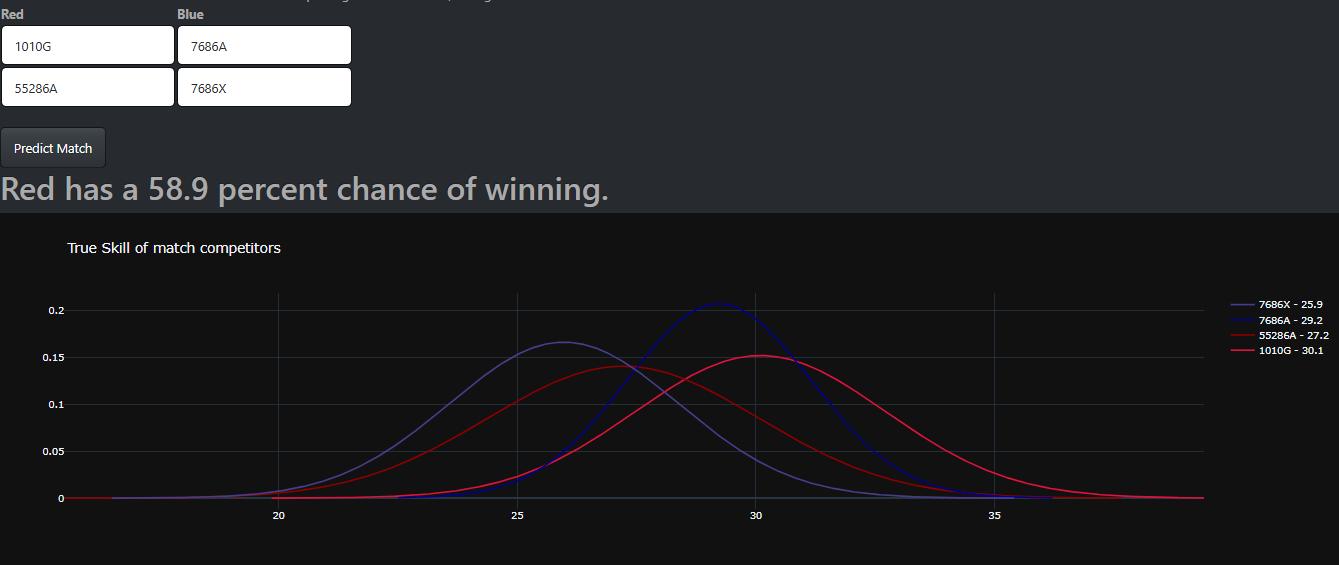
\includegraphics[width=0.8\linewidth]{images/SND.png}
    \caption{Caption}
    \label{fig:enter-label}
\end{figure}
\begin{itemize}
    \item \textbf{Blue Alliance:} 7686A - 7686X
    \item \textbf{Red Alliance:} 1010G - 55286A
    \item \textbf{Score}: \colorbox{cyan}{36}
    \colorbox{red}{6}
    \item \textbf{Autonomous Winner:} Blue
    \item \textbf{How the match went}: Autonomous Period: Red crossed, which makes Blue the winner. Driver: Blue quickly got both Positive Corners filled, which made them the winners from the start. Red would have to fill every other Mobile Goal, plus completely filling a Neutral Stake. which is what the attempted. When the Protected Period rolled around. Blue left the corners, took both full red Mobile Goals and put them in the Negative Corner. Which made them the victor of the match. What a crazy match, 1010G was undefeated until this point, beaten by two South Dakota teams.
\end{itemize}
\subsection*{Finals 1}
\subsubsection*{Prediction}
\begin{figure}[H]
    \centering
    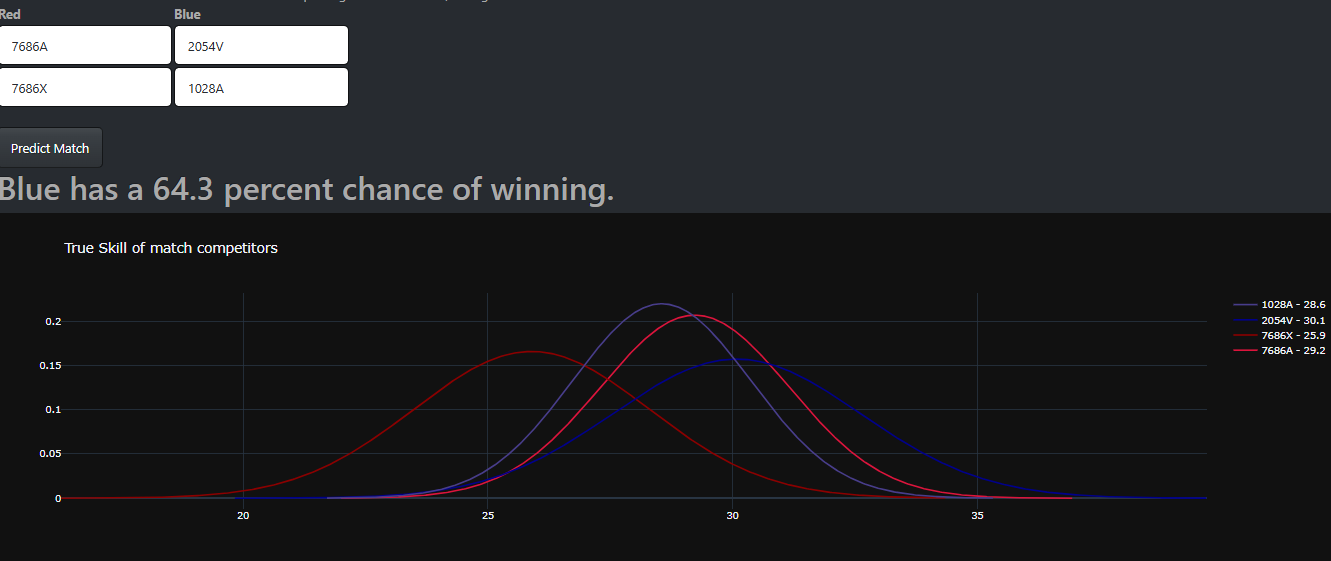
\includegraphics[width=0.8\linewidth]{images/FND.png}
    \caption{Finals Predictions}
    \label{fig:enter-label}
\end{figure}
\begin{itemize}
    \item \textbf{Blue Alliance:} 2054V - 1028A
    \item \textbf{Red Alliance:} 7686A - 7686X
    \item \textbf{Score}: \colorbox{cyan}{39}
    \colorbox{red}{31}
    \item \textbf{Autonomous Winner:} Tie
    \item \textbf{How the match went}: Autonomous Period: Both Alliances had the exact same Autonomous, so they tied in that regard. Driver: Red got a full Mobile Goal in a Positive Corner, Blue did the same. They ended up getting both top Rings on Neutral Stakes
\end{itemize}
\subsection*{Finals 2}

\begin{itemize}
    \item \textbf{Blue Alliance:} 2054V - 1028A
    \item \textbf{Red Alliance:} 7686A - 7686X
    \item \textbf{Score}: \colorbox{cyan}{32}
    \colorbox{red}{35}
    \item \textbf{Autonomous Winner}: Blue
    \item \textbf{How the match went}: 7686A crossed the Autonomous line, so Blue Alliance won. Driver: 7686X got A's Mobile Goal, and put it in the corner, the entire match 1028A was trying to score a Ring on the Mobile Goal, but 7686X wouldn't let them, Chase saved the Neutral Stake at least half a dozen times, at the final second, Chase ended up scoring a Ring on the Neutral Stake, if this hadn't happened, we would've lost, and we would go home.
\end{itemize}
\subsection*{Finals 3}
\subsubsection*{Prediction}

\begin{itemize}
    \item \textbf{Blue Alliance:} 2054V - 1028A
    \item \textbf{Red Alliance:} 7686A - 7686X
    \item \textbf{Score}: \colorbox{cyan}{0}
    \colorbox{red}{30}
    \item \textbf{Autonomous Winner}: Red
    \item \textbf{How the match went}: Autonomous Period: Red missed a Ring, but Blue missed two, so Red won. Driver: Blue had gotten both Mobile Goals in a Positive Corner. It looks like they were going to be the winner, but in the Protected Period, 2054V attached to one of their Mobile Goals in the Positive Corner, and disqualified themselves. Making 7686X and 7686A the tournament winners.
\end{itemize}
\begin{figure}[H]
    \centering
    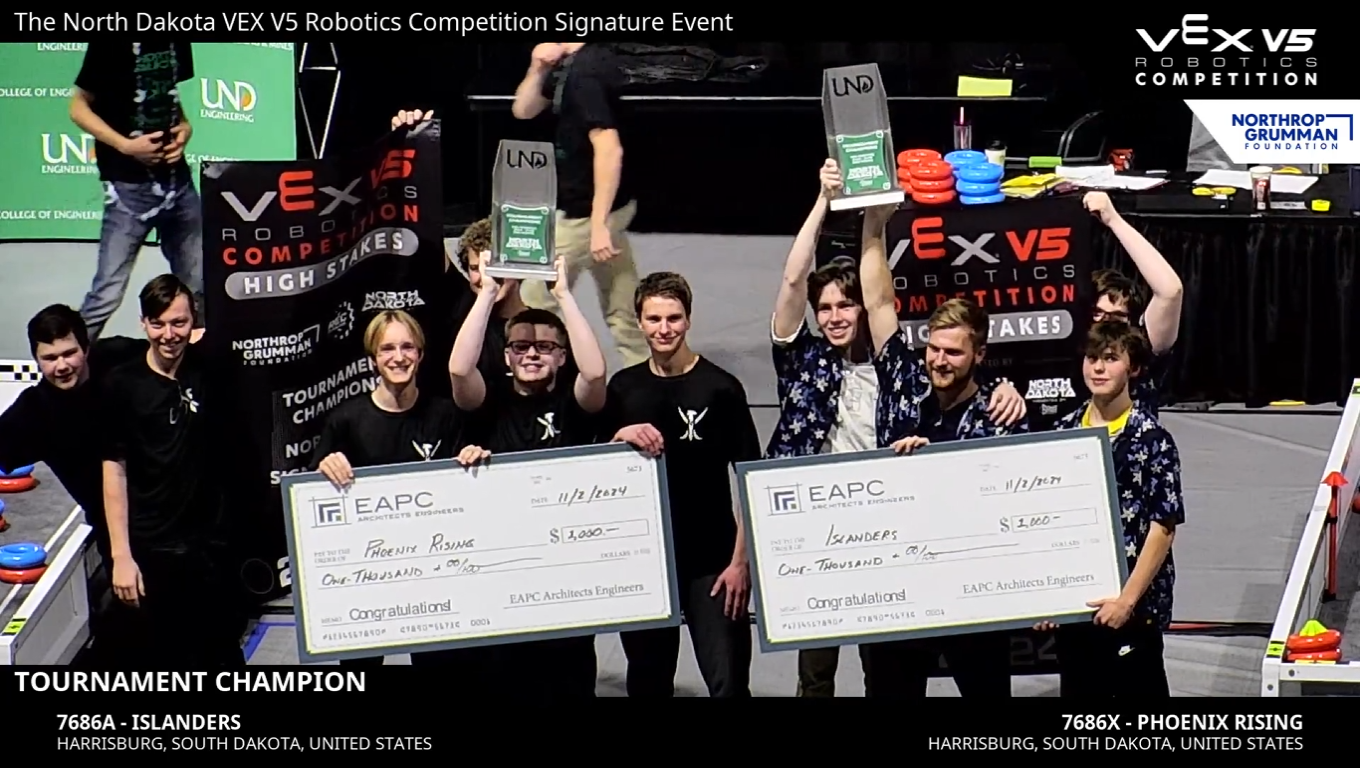
\includegraphics[width=0.8\linewidth]{images/streampicture.png}
    \caption{Tournament Champions}
    \label{fig:tournamentchamps}
\end{figure}
\section*{Lessons Learned}
\begin{itemize}
    \item \textbf{Overall Record For North Dakota}: 7/9/0 44\%
    \item \textbf{Overall Record for High Stake}: 11/13/0 46\%
\end{itemize}
Our next tournament is in Harrisburg, South Dakota on November 23rd. We want to start building Robot V2.0 at this time, no matter what we would not use this robot for November 23rd. While Connor is building V2.0, Chase will be driving V1.4. 

\white{Grand Forks Signature Event Reflection (November 3rd, 2024)}
\chapterauthor{Ian Smith}
\info{Ian Smith}{Grand Forks Signature Event}{November 3, 2024}
\subsection*{Inspection Period Lesson}
Throughout the Grand Forks signature event, the team learned a significant amount about high-level judging. After some critical thinking, improvements can be made. Discussing in chronological order, the team first found out during the inspection period by a head referee (who was extremely qualified) that there was some illegal anti-slip material on the claw. This should be taken as a lesson that the team cannot trust that every item within the organization is VEX official. 

The problem, however, was something that everyone on the team had overlooked. The referee caught the mistake by pointing out the specific pattern in the material. The official part can be found here SKU (275-0121) \cite{vexRobotics}. The solution was to add rubber bumpers in its place, which happened to work even better than the original material. After making this change, the team was able to easily pass inspection.

\subsection*{Judges Interview Analysis}
About halfway through day one, the team received an interview with the judges. Throughout the interview, the goals were to maintain good engagement, use the engineering design process (EDP), go in-depth with explanations while maintaining engagement, and ensure engagement from everyone on the team during the interview.

\begin{figure}[h!]
    \centering
    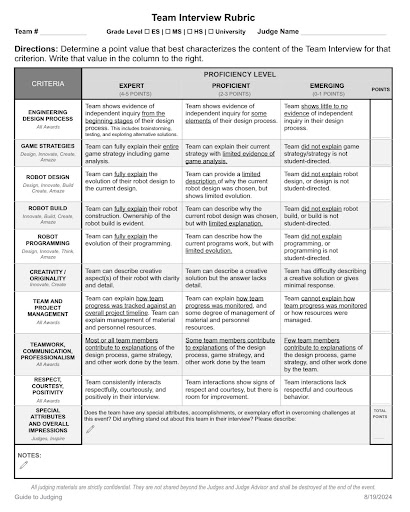
\includegraphics[width=0.8\textwidth]{images/teaminterviewrubric}
    \caption{Team Interview Rubric}
    \label{fig:team-interview-rubric}
\end{figure}

\begin{center}
\begin{tabular}{|l|c|}
\hline
\textbf{Category} & \textbf{Score} \\
\hline
EDP & 4 \\
Game Strategies & 3 \\
Robot Design & 5 \\
Robot Build & 5 \\
Robot Programming & 4 \\
Originality & 5 \\
Management & 2 \\
Soft Skills & 3 \\
Attitude & 5 \\
Special Impressions & 5 \\
\hline
\end{tabular}
\end{center}

Having access to the judging rubric from the guide to judging \cite{rubricForJudgingInterviews}, the team graded how the interview went. Tying in the engineering design process to the interview, build and test happened simultaneously. The goal of this analysis is to improve the next build and test with the current "generate concepts" stage.

After analyzing the table, the team did well in the interview but failed to explain proper project management. The team could certainly improve game strategies and soft skills scores dramatically by going into more depth. Overall, the team had a good interview but failed to go in-depth on the people management side of the team.

\subsection*{Notebook Clarification}
Before performing analysis for the notebook, it is crucial to discuss a critical event that took place due to some unclear wording in one section of the notebook. Although extra effort and attention were put into the chapter on CNC machining, the judges still thought that the team was using outside material in place of the official VEX parts listed.

As clarification, this is not true, and the team strictly uses only VEX parts bought directly from either Robosource or VEX. As stated in the updated clarification at the end of the chapter, this was strictly research and material identification derived from the VEX website \cite{vexRobotics} and the Machinists Handbook \cite{machinists}. Because of concern regarding \textless R2\textgreater, if machining were to be implemented, Ian would thoroughly document the process and create video evidence to show that students were the only ones doing the work.

\subsection*{Notebook Analysis}
As for the actual judging of the notebook and the team’s independent grading, being confronted about machining implies that the notebook was deemed developed because the judges read it in-depth. The grading was based on this document \href{https://v5rc-kb.recf.org/hc/en-us/articles/9681296966423-Guide-to-Judging-Judging-Engineering-Notebooks}{Guide to Judging Engineering Notebooks} and this document \href{https://kb.roboticseducation.org/hc/en-us/articles/4461349729047-Judging-Resource-Engineering-Notebook-Rubric}{Judging Resources Engineering Notebook}.

\begin{figure}[H]
    \centering
    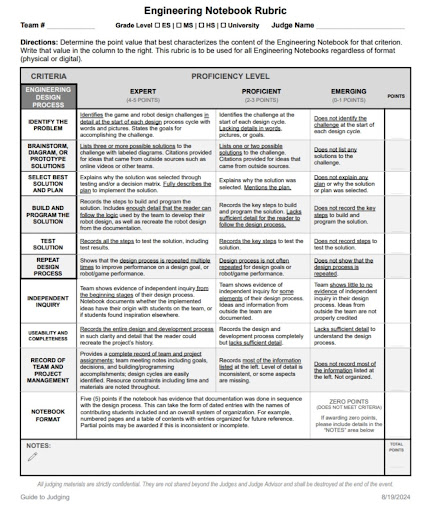
\includegraphics[width=0.8\textwidth]{images/engineeringnotebookrubric}
    \caption{Engineering Notebook Rubric}
    \label{fig:engineering-notebook-rubric}
\end{figure}

\begin{center}
\begin{tabular}{|l|c|}
\hline
\textbf{EDP Step} & \textbf{Score} \\
\hline
Identify the Problem & 4 \\
Prototype the Solution & 4 \\
Select Solution and Draft & 4 \\
Build and Program & 3 \\
Test & 3 \\
Repeat & 4 \\
Independent Inquiry & 5 \\
Usability and Completeness & 4 \\
Management & 5 \\
Format & 5 \\
\hline
\end{tabular}
\end{center}

The team didn’t score badly on most of the notebook grading. However, separate areas were identified that could be drastically improved upon:
\begin{itemize}
    \item Length and depth of answers.
    \item Ensuring all stages of the EDP are fully documented and followed. This is more of a depth of documentation issue rather than a “not using the EDP” issue.
    \item Ensuring all uses of outside sources are cited. Some citations exist but not enough.
    \item Revising the Innovate submission and treating the AI chapter and the simulator chapter as more of a reference to a separate EDP rather than the whole submission.
\end{itemize}

Overall, after some revision, the team could win many judged awards this season. The main revisions that need to happen are depth of analysis and including more relevant content. The self-judged score before revision was 82/100.
